\documentclass[../main.tex]{subfiles}
\begin{document}
	\begin{theorem}[о расстоянии до линейного подпространтсва]
		$L = span(\underset{\text{базис}}{a_1 \ldots a_k}), x = y + z, y \in L, z \in L^\perp \Rightarrow dist^2(x, L) = \|z\|^2 = \mathlarger{\frac{g(a_1 \ldots a_k, x)}{g(a_1 \ldots a_k)}} \neq 0$
	\end{theorem}
	\begin{proof}
		$\underbracket{a_1 \ldots a_k}_\text{лин. нез.} x \underset{\text{Г-Ш}}{\leadsto} \underset{\text{попарно-ортог.}}{b_1 \ldots b_k b_{k+1}} \Sspace span(a_1 \ldots a_k) = span(b_1 \ldots b_k)\n
		b_{k+1} = x - \underbrace{\sum\limits_{i=1}^k c_i b_i}_{\stackrel{||}{y \in L}} \Rightarrow b_{k+1} = x-y = z \underset{\text{Т-ма о } det \text{ матрицы } G \text{(следствие)}}{\Rightarrow}
		\|b_{k+1}\|^2 = \|z\| = \mathlarger{\frac{g(a_1 \ldots a_k, x)}{g(a_1 \ldots a_k)}}$
	\end{proof}
	\underline{Упражнения}:
	\begin{mylist}
	\item
	\begin{minipage}[t]{0.6\textwidth}
		$P = x_0 + L$ линейное многообразие \\
		$dist (x, P) = \min\limits_{u\in P} \|x - u\| \overset{\text{доказать}}{=} \|z\| = \sqrt{\mathlarger{\frac{g(a_1 \ldots a_k, x-x_0)}{g(a_1 \ldots a_k)}}}\n
		L = span(a_1 \ldots a_k)\slide{0.2\textwidth} x - x_0 = \underset{\in L}{y}+z$
	\end{minipage}
	\begin{minipage}[t]{0.3\textwidth}
	\vspace{0pt}
	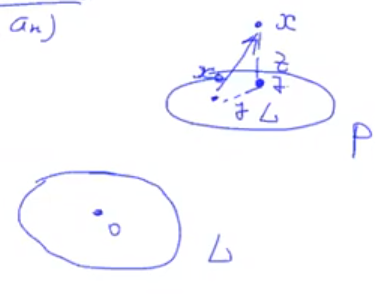
\includegraphics[width=180px]{pic25}\end{minipage}\\
	\item
	\begin{minipage}[t]{0.6\textwidth}
	$P_1, P_2 \Sspace P_i = x_i + L_i \Space i = 1, 2\n
	dist(P_1, P_2) = \min\limits_{\stackrel{\mathlarger{u_1 \in P_1}}{u_2 \in P_2}} \|u_1 - u_2 \| \overset{\text{доказать}}{=} \|z\|\n
	x_2 - x_1 = \underset{\in L_1 + L_2}{y} + \underset{\in (L_1 + L_2)^\perp}{z}$
	\end{minipage}
	\begin{minipage}[t]{200px}
		\vspace{0pt}
		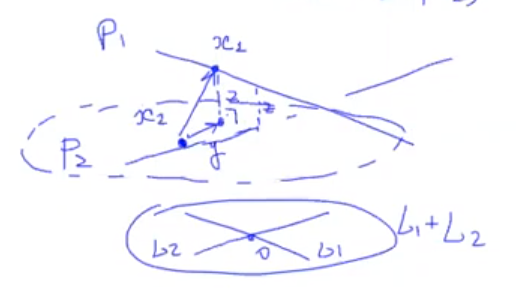
\includegraphics[width=200px]{pic26}
	\end{minipage}\\
	\end{mylist}
	\begin{defin}
		$\underset{\text{Лин. подпр.}}{L_1 \ldots L_k} \subset V$ называются \underline{попарно-ортог.}, \\если $\forall x_i \in L_i \Space \forall x_j \in L_j \Space (x_i, x_j) = 0 \Space i\neq j$\n
		Очевидно, $L_1 \ldots L_k$ дизъюнктны.\n
		$\underset{x_i \in L_i}{x_1 + \ldots + x_k} = \0 \Space |\cdot x_j \; \; j = 1\ldots k \; \; \; 
		\begin{matrix}
			(\sum\limits_{i=1}^k x_i, x_j) &= 0\\
			||\\
			\sum\limits_{i=1}^k (x_i, x_j)& = (x_j, x_j) &=0 \Leftrightarrow x_j = \0
		\end{matrix}$
	\end{defin}
	\begin{defin}
		$L_1 \ldots L_k$ попарно ортог. $\Space V = \bigoplus\limits_{i=1}^k L_i \Space \underset{\text{проекторы}}{\p_i: V \rightarrow L_i} \Space \begin{matrix}
			\text{\underline{операторы ортогонального}}\\\text{\underline{проектирования}}
		\end{matrix}\n
		\forall x \in V \Space x = \sum\limits_{i=1}^k \underset{\in L_i}{x_i} = \sum\limits_{i=1}^k \p_i x \Space \text{(однозн. предст.)} $\n
		$\boxed{x_i = \p_i x}$ -- \underline{ортог. проекция $x$} на подпространство $L_i$ 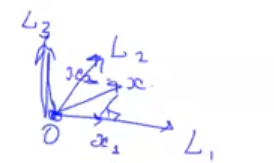
\includegraphics[width=100px]{pic27}\n
		$\boxed{(x_i, x_j) = 0 \; \; i\neq j} \Rightarrow$ по т-ме Пифагора $\boxed{\|x\|^2 = \sum\limits_{i=1}^k \|x_i\|^2}$ 
	\end{defin}
	$e_1 \ldots e_n$ ортогональный базис. $\Space L_i = span(e_i)\n
	V = \bigoplus_{i=1}^n L_i \Space \underset{\stackrel{\updownarrow}{\mathlarger{x = \sum\limits_{i=1}^n x_i e_i}}}{\forall x \in V:} x = \underset{\stackrel{\updownarrow}{\text{ортог. проекция на }e_i \text{ -- вектор}}}{\sum\limits_{i=1}^n \underset{\in L_i}{x_i}} = \sum\limits_{i=1}^n x_i e_i \Space $
	$\begin{matrix}x_i \text{ -- координата относительно } e_i,\\ \text{проекция элемента } x \text{ на } e_i \end{matrix}$\n
	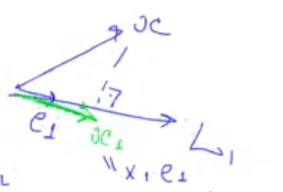
\includegraphics[width=130px]{pic28}\n
	$\forall j = 1 \ldots n \Space (x, e_j) = (\sum\limits_{i=1}^n x_i e_i, e_j) = \sum\limits_{i=1}^n x_i \underset{\stackrel{||}{0 \; i\neq j}}{(e_i, e_j)} = x_j (e_j, e_j)\n
	\Rightarrow \boxed{x_j = \frac{(x, e_j)}{e_j, e_j}}$ -- коэфф--ты Фурье вектора $x$ относительно базиса $e$ (ортогон.)\n
	$\begin{matrix}x \overset{?}{\leftrightarrow} \sum\limits x_j e_j\\
	x = \sum x_j e_j \end{matrix}$ -- в бесконечномерных пространствах не все так просто, но мы этим и не занимаемся.\n
	$\boxed{\|x\|^2 = \sum\limits_{i=1}^n \|x_i\|^2 = \sum\limits_{i=1}^n |x_i|^2 \|e_i\|^2}$ \underline{Тождество Парсеваля}\n
	$\boxed{1 \leq k \leq n \Sspace \sum\limits_{i=1}^k |x_i|^2 \|e_i\|^2 \leq \|x\|^2}$ \underline{Неравенство Бесселя}\n
	"Квадрат длины вектора не меньше суммы квадратов длины его проекций"\n
	$e_1 \ldots e_n$ \dunderline{о.н.б.} $V \Space (e_i, e_j) = \delta_{ij}\n
	\boxed{x_i = (x, e_i)} \begin{matrix}
		\text{ -- коэффициенты } x \text{ относительно } e\\
		\text{ -- коэффициенты Фурье}\\
		\text{ -- проекция на } e_i
	\end{matrix}\n
	\boxed{\|x\|^2 = \sum\limits_{i=1}^n |x_i|^2}$ -- тождество Парсеваля \Sspace $\sum\limits_i^k |x_i|^2 \leq \|x\|^2$ -- неравенство.\n
	$V = \bigoplus\limits_{i=1}^k L_i \Space L_i$ попарно-ортогональны $\Space \p_i: V \rightarrow L_i$\\
	$\Sspace V = span(\underbrace{e_1}_{L_1} \ldots \underbrace{e_n}_{L_k})$ о.н.б.\n
	$\Rightarrow \forall x \in V \; \boxed{x_i = \p_i x = \sum\limits_{e_j \in L_i} (x, e_j) e_j}$
	\subsection{Изометрия унитарных (евклидовых) пространств. Теорема Рисса. Естественный изоморфизм евклидового пространства и сопряженного к нему.}
	\begin{defin}
		\underline{Изометрией} называется изоморфизм линейных пространств с сохранением скалярного (псевдоскалярного) произведения.\\
		$(V, (\cdot, \cdot)_V) \Space (V', (\cdot, \cdot)_{V^*})$ унит. (евкл.) $\Space V \cong V^*\n
		\forall\; \begin{matrix}
			x, &y &\in V\\
			\updownarrow & \updownarrow\\
			x', &y &\in V' 
		\end{matrix} \; \; \boxed{(x, y)_V = (x', y')_{V'}}$\n
		Очевидно, при изометрии сохраняется расстояние:\n
		$\|x-y\|^2_V = (x-y, x-y)_V = (x'-y', x'-y')_V' = \|x-y\|^2_V$\n
		"Изометрия $\equiv$ сохраняет метрику"
	\end{defin}
	\begin{theorem}[об изометрии]\ \\
		Любые 2 унитарных (евкл.) пространства одной размерности изометричны.
	\end{theorem}	
	\begin{proof}
		$\forall $ 2 лин. пространства одной размерности изоморфны \Space $V \cong V'$\n
		См. 1 семестр. \Space $\begin{matrix}
			e_1 \ldots e_n \; V\\
			\text{базис о.н.б.}\\
			e'_1 \ldots e'_n \; V'\\
			\text{базис о.н.б.}
		\end{matrix} \Space \begin{matrix}
			\underset{\in V}{x} = \sum x_i e_i \leftrightarrow \underset{\in V'}{x'} = \sum x_i e'_i\\
			\text{было доказано, что это изоморфизм}
		\end{matrix}\n
		(x, y)_V = \sum\limits_{i=1}^n x_i \vec y_i = (x', y')_{V'} \Rightarrow \text{ изометричны.}$
	\end{proof}
	$(V, (\cdot, \cdot)) \Space V^*$ -- сопряженное к $V$\n
	Фиксируем $y \in V \Rightarrow \forall x \in V \Space \boxed{f(x):= (x, y)} \Space \underset{\text{линейное отображение}}{f: V \rightarrow K} \Rightarrow f \in V^*\n
	\boxed{\begin{matrix}\forall y \in V \leadsto f \in V^*\\
		\stolead ?
	\end{matrix}}$
	\begin{theorem}[Рисса $(V(\cdot, \cdot)$]\ \\
		$\forall f \in V^* \; \exists! y \in V: \forall x \in V \; f(x) = (x, y) \Space y$ -- \underline{присоединенный вектор} к $f$ 
	\end{theorem}
	\begin{theorem}\ \\
		\textbf{Единственность: } $\pu y': f(x) = (x, y) \; \forall x \in V\n
		\Rightarrow \{\forall x \in V \Space \0 = f(x) - f(x) = (x, y) - (x, y') = (x, y-y')\} \Leftrightarrow y - y' = \0 \Leftrightarrow y = y'$\n
		\textbf{Существование: } $\pu e_1 \ldots e_n$ о.н.б. $V \Space f \in V^* \Space \forall x \in V \; \; x = \sum\limits_{i=1}^n x_i e_i \n
		\Rightarrow f(x) = \sum\limits_{i=1}^n x_i f(e_i) \Sspace y_i = \vec{f(e_i)} \Space y = \sum\limits_{i=1}^n y_i e_i \n
		\Rightarrow \forall x \in V \Space f(x) = \sum\limits_{i=1}^n x_i \vec y_i \underset{\stackrel{\updownarrow}{\text{скал.(псевдоск.) про. в о.н.б.}}}{=} (x, y)$
	\end{theorem}
	$\boxed{\begin{matrix}
			V \leftrightarrow V^*\\
			\text{те-ма Рисса}\\
			\text{будет ли изоморфизм? Будет ли изометрия?}
		\end{matrix}}$\n
	$V \underset{\text{т-ма Рисса}}{\longleftrightarrow} \; \; $ 
	$\begin{matrix}\text{\underline{изоморфизм}, если }V\text{  евклидово пространство,}\\ \text{\underline{не изоморфизм}, если }V\text{ унитарное пространство.} \end{matrix}$\n
	Изоморфизм именно в смысле теоремы Рисса!\n
	$y_1, y_2 \in V \underset{\text{т-ма Рисса}}{\leftrightarrow} f_1, f_2 \in V^* \Space \underset{\forall x \in V}{f_i(x) = (x, y_i)} \; i = 1, 2\n
	\underset{\lambda \in K}{y_1 + \lambda y_2} \in V \stolead (x, y_1 + \lambda y_2) = \underbracket{(x, y_1)}_{f_1(x)} + \vec \lambda \underbracket{(x, y_2)}_{f_2(x)}\n
	y_1 + \lambda y_2 \leftrightsquigarrow f_1 + \vec \lambda f_2\n
	\boxed{\begin{matrix}
			V \text{ евклидово пространство} \Sspace V \cong V^* \Leftrightarrow \begin{matrix}
				y \in V \leftrightarrow f \in V^*\\
				\forall x \in V: f(x) = (x, y)
			\end{matrix}\\
			\text{\underline{Естественный изоморфизм}}
		\end{matrix}}$\n
	$V^*$ дадим определение $(f, g)_{V^*} := (y, z) \Space \text{1-4 скал. произведения вып.} \Rightarrow \text{\dunderline{Изометрия}}\n
	\begin{matrix}
		V^* \ni f \leftrightarrow y \in V\\
		V^* \ni g \leftrightarrow z \in V
	\end{matrix} \slide{150px} \boxed{\begin{matrix}
			V \cong V^*\\
			(\cdot, \cdot) \Space (\cdot, \cdot)_{V^*}
		\end{matrix}}\n
	e_1 \ldots e_n$ о.н.б. $V \underset{\text{т-ма Рисса}}{\leftrightarrow} \omega^1 \ldots \omega^n$ сопряженный базис $V^*$\n
	\underline{Действительно}, $\omega^i(x) = x^i = (x, e_i) \underset{\text{т-ма Рисса}}{\leftrightarrow} e_i \leftrightarrow \omega^i$
	\subsection{Тензоры в евклидовом пространстве. Метрический тензор. Взаимные базисы. Операции поднятия и опускания индексов.}
	$V$ линейное вещ. про-во \Space $(\cdot, \cdot)$ скалярное про-е \Sspace $V$ евклидово пространство\n
	$e_1 \ldots e_n$ базис $\Sspace \Gamma = \underset{\text{матрица Грама}}{G(e_1 \ldots e_n)} = ((e_i, e_j))_{n\times n} = (g_{ij})_{n\times n}\n
	\Gamma \in T_{(2, 0)}$ -- \underline{метрический ковариантный тензор}\n
	$e'_1 \ldots e'_n$ базис. $\Sspace \Gamma' = ((e'_i, e'_j))_{n\times n} = (g'_{ij}) \Space T = T_{e\rightarrow e'} = (t^i_j) \Rightarrow\n
	\underset{\text{было док-во}}{\Rightarrow} \Gamma' = T^T \Gamma T \Leftrightarrow g'_{ij} = 
	t^k_{ij} = t^k_i g_{kl} t^l_j = g_{kl}t^k_i t^l_i \Rightarrow \Gamma$ -- $(2, 0)$ тензор.
	\begin{stat}
		$\Gamma^{-1}$ тензор типа $(0, 2)$
	\end{stat}
	\begin{proof}
		$\pu \; \Gamma^{-1} = (g^{ij})_{n\times n} \Space S = T^{-1} = (S^k_l)_{n\times n} \; \; T_{e\rightarrow e'}\n
		(\Gamma^{-1})' = (g'^{ij})_{n\times n} \Sspace (\Gamma^{-1})' = (\Gamma')^{-1} = (T^T \Gamma T)^{-1} = T^{-1} \Gamma^{-1} (T^{-1})^T = S \Gamma^{-1} S^T \Leftrightarrow\n
		\Leftrightarrow g'^{ij} = S^i_k g^{kl} S^j_l = g^{kl} S^i_k S^j_l \Rightarrow \Gamma^{-1}$ 2 контрвариантный тензор.
	\end{proof}
	\begin{defin}
		$\Gamma^{-1}$ тензор типа (0, 2) называется  \underline{контрвариантным метрическим тензором}
	\end{defin}
	\textbf{Свойства $\Gamma, \Gamma^{-1}:$}
	\begin{mylist}
		\item $\boxed{g_{ij} g^{jk} = \delta_j^k = g_{ji} g^{kj}} \Space (\Gamma \Gamma^{-1} = E = \Gamma^{-1} \Gamma)$
		\item 
		$\Gamma$ и $\Gamma^{-1}$ \underline{симметр. тензоры} $\Space (\Gamma = \Gamma^T \Rightarrow (\Gamma^{-1})^T = (\Gamma^T)^{-1} = \Gamma^{-1})$
		\item $\forall x, y \in V \Space \boxed{(x, y) = g_{ij} x^i y^j}$, причем $\boxed{\underset{\stackrel{||}{(x, x)}}{g_{ij}} x^i y^j > 0, \text{ если } x \neq 0}$
	\end{mylist}
\end{document}